\documentclass[fleqn,usenatbib]{mnras}

%%% DEBUG SETTINGS - remove at the end %%%%%%%%%%%%%%%
\usepackage{silence} % silence error warinings
\WarningFilter{caption}{Unsupported document class} % caption doesn't know mnras..
\hbadness = 5000
\vbadness = 10000
% \usepackage{}

% MNRAS is set in Times font. If you don't have this installed (most LaTeX
% installations will be fine) or prefer the old Computer Modern fonts, comment
% out the following line
%\usepackage{newtxtext,newtxmath} % not yet supported on arxiv and uni computer
%\usepackage{txfonts}

% Depending on your LaTeX fonts installation, you might get better results with one of these:
%\usepackage{mathptmx}
%\usepackage{txfonts}

% Use vector fonts, so it zooms properly in on-screen viewing software
% Don't change these lines unless you know what you are doing
\usepackage[T1]{fontenc} % make sure font is supported
% \usepackage{ae,aecompl} %obsolete when using modern fonts
\usepackage[final]{microtype} % make sure font is supported
% and a suitable font
\usepackage{lmodern} % use a modern font with T1 support
%\usepackage{cm-super} % use a modern font with T1 support


%%%%% AUTHORS - PLACE YOUR OWN PACKAGES HERE %%%%%

% Only include extra packages if you really need them. Common packages are:
%\usepackage[dvipdfmx]{graphicx}	% Including figure files
\usepackage{graphicx} % Including figure files
%\usepackage[skip=0pt]{subcaption}
\usepackage{amsmath}	% Advanced maths commands
\usepackage{amssymb}	% Extra maths symbols
\usepackage{pifont}	% Extra maths symbols
%\usepackage{bmpsize}  % PS still needs this for correct bounding boxes?


% TODO stuff, comment out for final submit
\usepackage{todonotes} % as long as we are editing...
%\usepackage{showframe} % for debug
%\overfullrule=5pt      % show overfull boxes

% I disabled hyperlink in the cls und included it here because of bugs
\usepackage{hyperref}   % Hyperlinks
\hypersetup{colorlinks=true,linkcolor=blue,citecolor=blue,filecolor=blue,urlcolor=blue}

\edef\smallwidth{0.4\linewidth}

\newcommand{\inclfig}[2]{
  \centering
	\includegraphics[width=\smallwidth]{spaghetti/#2_input}%
	\includegraphics[width=\smallwidth]{spaghetti/#2_img2}
	\includegraphics[width=\smallwidth]{spaghetti/#2_img1}%
	\includegraphics[width=\smallwidth]{img/M_encl/#2_M_encl}
	\includegraphics[width=\smallwidth]{spaghetti/#2_img3_ipol}%
	\includegraphics[width=\smallwidth]{masses/#1_#2_mstel_vs_mtot}
}

\newcommand{\inclfign}[2]{
  \centering
	\includegraphics[width=\smallwidth]{spaghetti/#2_input}%
	\includegraphics[width=\smallwidth]{spaghetti/#2_img2}
	\includegraphics[width=\smallwidth]{spaghetti/#2_img1}%
	\includegraphics[width=\smallwidth]{img/M_encl/#2_M_encl}
	\includegraphics[width=\smallwidth]{img/nsynth/#2_nsynth}%
	\includegraphics[width=\smallwidth]{masses/#1_#2_mstel_vs_mtot}
}

\newcommand*{\rot}{\rotatebox{90}}
\newcommand*{\OK}{\ding{51}}
\newcommand*{\NO}{\ding{55}}

\newcommand{\lenstitle}[1]{\noindent\textbf{#1} --}
\newcommand{\params}[3]{(\(\Theta_\text{E}:#1\), $\varepsilon:#2$, $\alpha_\varepsilon:#3$ )}

\newcommand{\asw}[1]{ASW000#1}
\newcommand{\sw}[1]{SW~#1}
\newcommand{\model}[1]{SL model~#1}

\newcommand{\figref}[1]{Figure \ref{fig:#1}}

\newcommand{\Mstel}{M_{\rm stel}}
\newcommand{\Mhalo}{M_{\rm h}}

\title[Short title, max. 45 characters]{Model of lens candidates from
  Space Warps CFHTLS}

% The list of authors, and the short list which is used in the headers.
% If you need two or more lines of authors, add an extra line using \newauthor
\author[R. Kueng et al.]{
Rafael Kueng,$^{1}$\thanks{E-mail: rafael.kueng@uzh.ch}
Presenjit Saha,$^{1}$
Lucy Oswald$^{3}$
%and Fourth Author$^{4}$
\\
% List of institutions
$^{1}$Physik Institut, University of Zurich, Winterthurerstrasse XXX, Zurich 8057, Switzerland\\
$^{2}$Department, Institution, Street Address, City Postal Code, Country\\
$^{3}$Another Department, Different Institution, Street Address, City Postal Code, Country
%$^{4}$Another Department, Different Institution, Street Address, City Postal Code, Country
}

% These dates will be filled out by the publisher
% \date{Accepted XXX. Received YYY; in original form ZZZ}

% Enter the current year, for the copyright statements etc.
\pubyear{2016}

% Don't change these lines
\begin{document}
\label{firstpage}
\pagerange{\pageref{firstpage}--\pageref{lastpage}}
\maketitle

\begin{abstract}
We report modelling follow-up of recently-discovered
gravitational-lens candidates in the CFHT Legacy Survey.  Lens
modelling was done by a small group of specially-interested volunteers
from the Space~Warps citizen-science community who originally found
the candidate lenses.  Models are categorised according to seven
qualitative and quantitive points.  Also included are some
improvements to the modelling software used (SpaghettiLens),
and discussion of strategies for scaling to future surveys
with more and frequent discoveries.

The candidates successfully modelled are all galaxies, with inferred
lensing masses ranging from $\sim10^{11}M_\odot$ to $>10^{13}M_\odot$.
Stellar masses have also been estimated, using photometry from the
CFHTLS pipeline and stellar-population models.  A trend well-known
in nearby galaxies, that star-formation efficiency is maximal for
total masses of $\approx10^{12}M_\odot$ and reduces for both lower and
higher masses, is discernable also in these much more distant
galaxies.
\end{abstract}

\begin{keywords}
gravitational lensing: strong -- keyword2
\end{keywords}

\section{Introduction}

Light deflection at the rim of the Sun is famously $1.75''$.  The
deflection angle can also be expressed in terms of the escape velocity
$2v_{\rm esc}^2/c^2$, with $v_{\rm esc}$ at the solar surface being
$\simeq620\rm\,km/s$.  The Galactic escape velocity at the Sun's
location is similar: $\approx500\rm\,km/s$, typical of massive
galaxies.  Thus, the outer regions of massive galaxies have lensing
deflections comparable to that at the rim of the Sun.  Yet these
quantitatively similar deflections have qualitatively different
consequences.  Light deflection by the Sun must be accounted for in
modern astrometry \citep[see e.g.,][]{2015CQGra..32p5008C} but is not
itself a physics probe in the way it was a century ago.  With distant
galaxies, however, light bending by $\sim1''$ introduces two new
phenomena.  First, for galaxies distant enough that their apparent
size is comparable to the bending angle, light deflection can cause
multiple images of background sources, or strong lensing.  Second, the
gravitational field is dominated by dark matter, hence strong lensing
becomes a probe of dark matter in galaxies.

With no unambiguous dark-matter particle detections so far, dark
matter has studied only through its indirect consequences on galactic
and larger scales.  In most work, dark matter is taken to be a
collisionless non-relativistic fluid (cold dark matter or CDM); in
recent years, the simulation by \cite{2005Natur.435..629S} has been
particularly influential in studying the formation of CDM structures.
Other scenarios have also been considered, such as a cold condensing
boson fluid \citep{2016ApJ...818...89S}.  There is a general
consensus, however, that the origins of galaxy lie in the
gravitational collapse, fragmentation, and mergers of dark-matter
clumps, into which fell gas, cooling through radiative processes to
form dense clouds and eventually stars.  There is, however, much
debate about the details, of which \cite{2012RAA....12..917S} provide
a nice summary.

Strong-lensing galaxies are a useful source of information on the
mutual dynamics and dark matter and gas in galaxies.  The topic has
been explored in several studies
\citep{2009ApJ...703L..51K,2011ApJ...740...97L,2012MNRAS.424..104L,
  2016MNRAS.459.3677L,2016MNRAS.456..870B} but it is desirable to
enlarge the samples from tens of lensing galaxies to thousands.  Doing
so requires finding more lenses, of course, but also modelling their
masses.

Recent searches through the CFHTLS \citep{2012SPIE.8448E..0MC} using
arc-finders
\citep{2012ApJ...749...38M,2014A&A...567A.111M,2014ApJ...785..144G} by
machine learning \citep{2016arXiv160504309P} and by visual inspection
by a citizen-science volunteers
\citep[Space~Warps][]{2016MNRAS.455.1191M} have between them
discovered an average of four lenses per square degree.  So one can be
optimistic about finding many thousands of lenses in the next
generation of wide-field surveys.  The expected flood of new lens
discoveries will need a similarly huge modelling modelling effort to
reconstruct their mass distributions.

To prepare for the challenge of massive-sample lens modelling,
\cite{2015MNRAS.447.2170K} developed a new modelling strategy,
implemented as the SpaghettiLens system.  The idea is to collaborate
with experienced members of the citizen-science community, who have
already participated in lens discovery through Space~Warps, as well as
several other projects involving astronomical data.  The style of
collaboration differs, however, from Space~Warps itself.  Space~Warps
works by sourcing a simple task to very large crowd

2016MNRAS.455.1171M,


One idea for coping with the challenge of modelling many more lenses
is to enlist the help of citizen scientists, a comm



 have between them discovered an average of








\section{Lens Modelling}


\subsection{Additional / Improved Synthetic Image}

Volunteers often ask about better indicators to identify wether the modelling resulted in a ``good'' or ``bad'' model.
We developped a prototype of a better syntetic image than just the rendering of a \todo{insert currently used source profile} profile.
It operates on the composite input image.
The user has to mask the supposed lensed images.
The algorith then establishes a grid on the source plane and projects the masked pixels of the lense plane back to the source plane.
Multiple lens plane pixels fall onto one source plane pixel and get averaged.
The new synthetic image then reverses the mapping, coloring each pixel in the lens plane with the corresponding values of the source plane pixel.

\begin{figure}
  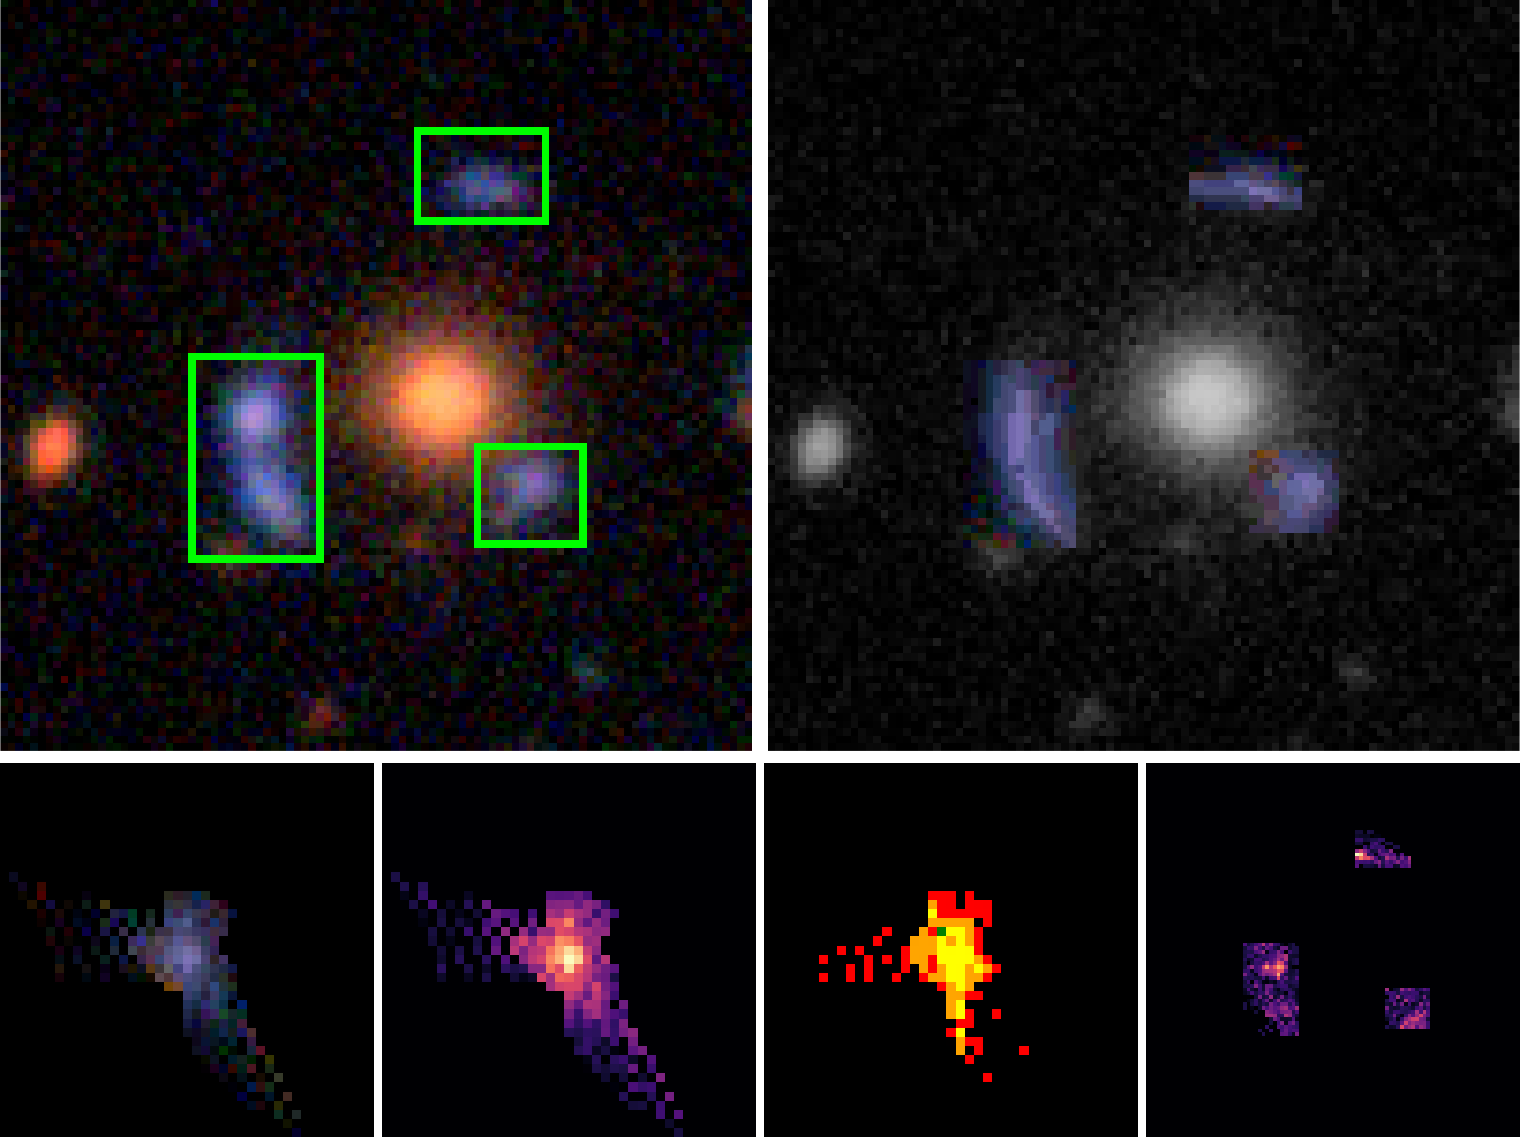
\includegraphics[width=\linewidth]{img/new_synth_img_detailed}
  \caption{
      Top-left: Orginal image, top-right: improved synthetic image for candidate \sw{5} (\asw{7k4r}) and model \model{12402};
      bottom from left to right:
        reconstructed source in color,
        intensity (grayscale),
        count of lens plane pixels per source plane pixel,
        residual of orginal image to improved syntetic image in grayscale
    }
  \label{fig:synthimg}
\end{figure}

\subsection{HiRes / Subsampling of central region}
In a previous paper \cite{2015MNRAS.447.2170K} we identified the problem of the tendency of the models to be too shallow.
We pinned down the problem to the central region and are confident to have it fixed with enabling sub pixel sampling in the central area.
The software allows for subsampling parameters of radius of pixels $r_\text{subs}$ and amount of subpixels per pixel $n_\text{subs}$.
\figref{subsampling} shows the results of different settings for $r_\text{subs}$ and $n_\text{subs}$.
We can see that even the computationally least expensive settings of $r_\text{subs}=1$ and $n_\text{subs}=3$ leads to drastically improved profiles.

\begin{figure}
  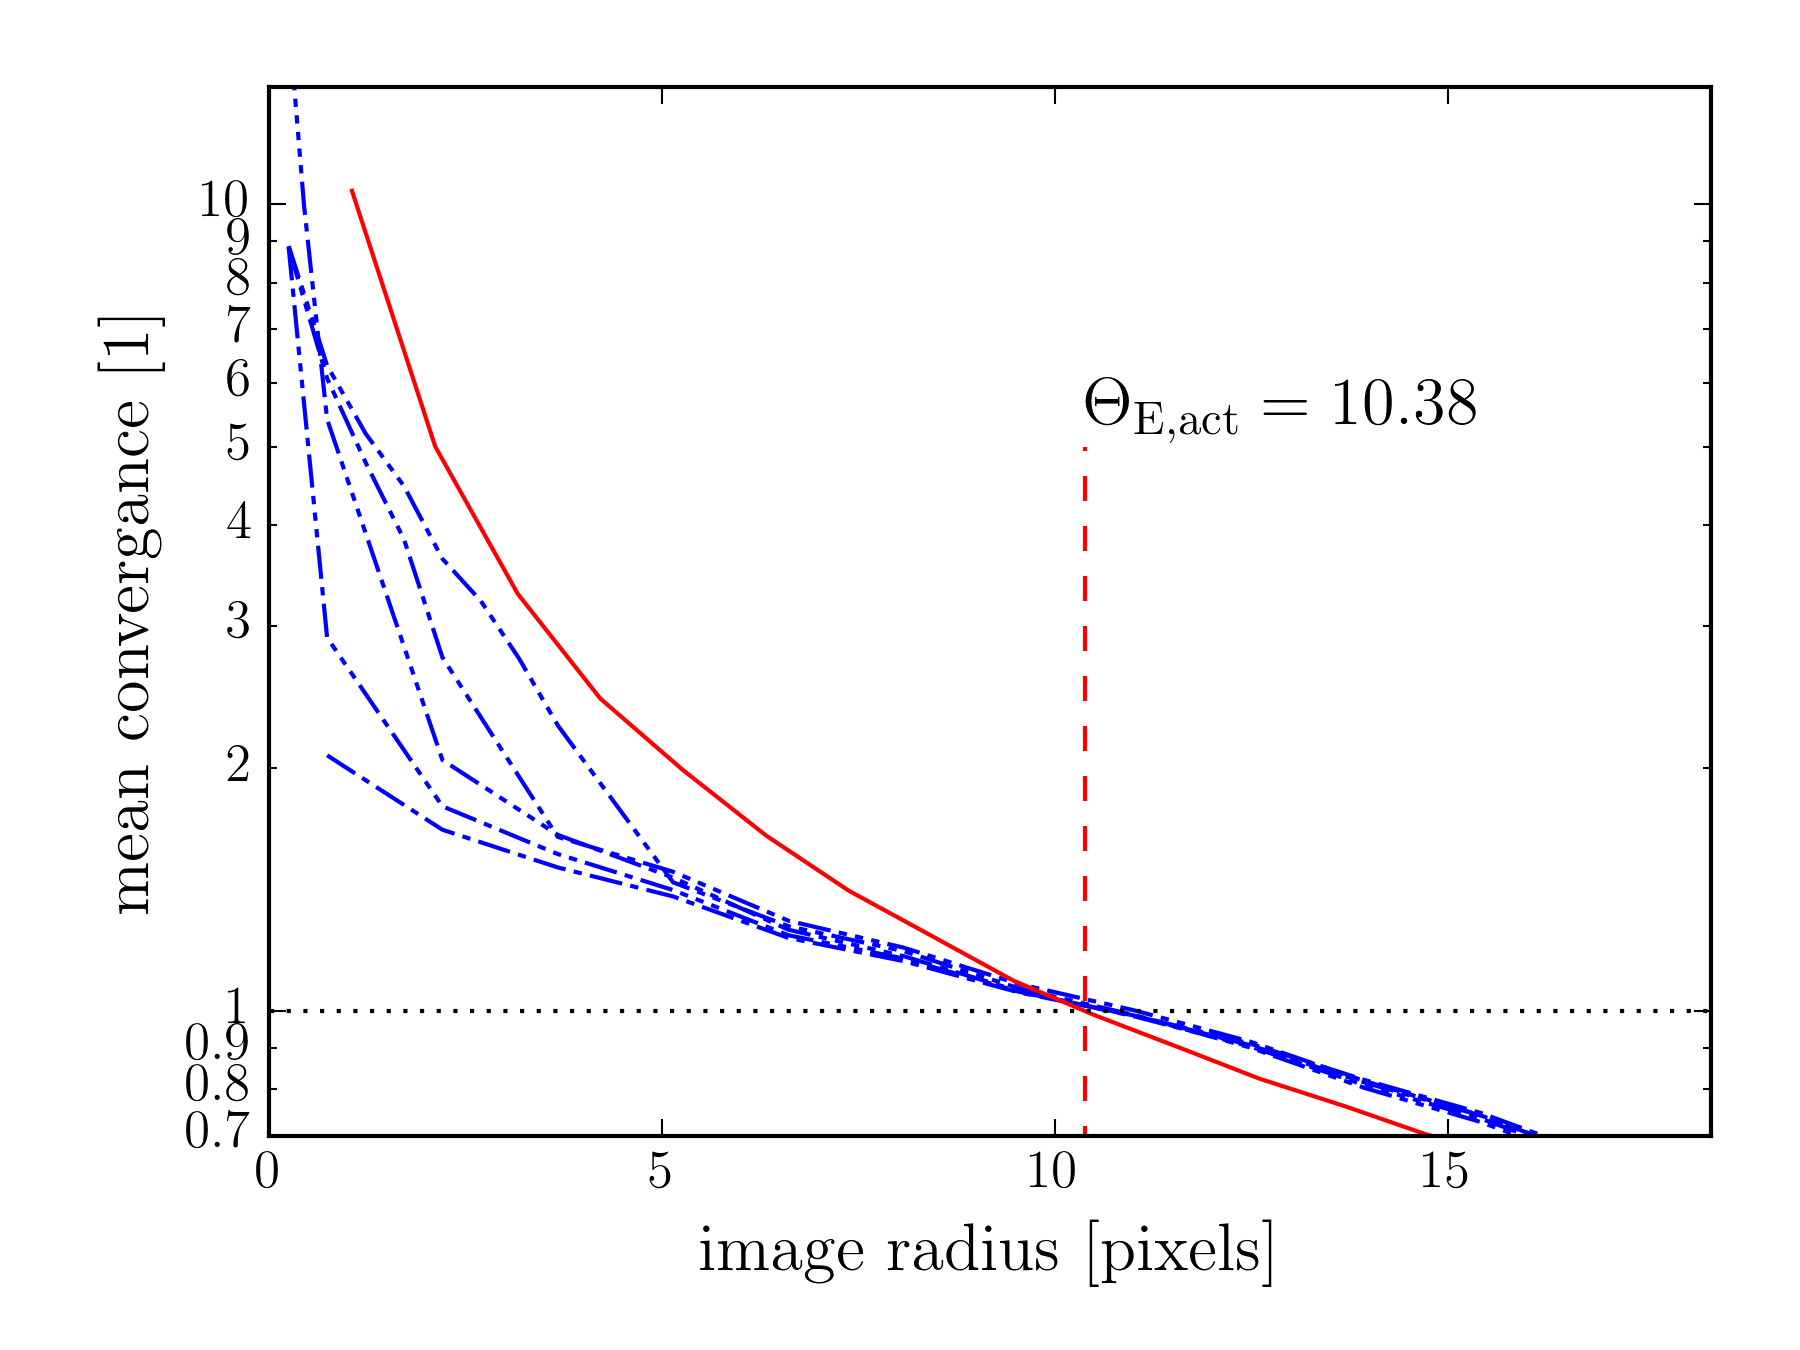
\includegraphics[width=\linewidth]{hires/007022_kappa_encl}
  \caption{
    Circularly averaged mass profile for different subsampling of central region.
    Red line without subsampling, blue lines show subsampling with dash-dot pattern showing the mode.
    $\cdot / \cdot \cdot \cdot$: $r_\text{subs}=1$ inner pixels, each subdivided into $n_\text{subs}=3$ sub pixels.
    $\cdot / \cdot \cdot \cdot \cdot \cdot$: $r_\text{subs}=1$, $n_\text{subs}=5$.
    $\cdot \cdot / \cdot \cdot \cdot $: $r_\text{subs}=2$, $n_\text{subs}=3$.
    $\cdot \cdot \cdot / \cdot \cdot \cdot $: $r_\text{subs}=3$, $n_\text{subs}=3$.
    }
  \label{fig:subsampling}
\end{figure}

\subsection{Parameterisation of pixel models} \label{sec:parameter}
In order to fit the set of pixelated models to a single parameterised model, a program was written that took a parameterised function and subtracted from it the mean and the principle components of the data, which were calculated using classical Principle Component Analysis.
This created the residuals function.
The number of components defined as principle was varied to test how this affected the output, and it was found that using 5 principle components tended to give a reasonable approximation.
A masking function was added which selected only the data points that fell inside the image of the lens, and the principal components were clipped in order to keep the values inside the region of the ensemble of models.
Any value higher than the clip was set to be the clip value.
This was chosen to be 2.5 as, assuming that the data follows a Gaussian error distribution, almost all the values for the variance should lie between 2 and 3 standard deviations from the mean.
Minimising the residuals function produces the set of parameters that fit the parameterised function to the original pixelated ensemble most closely.
A least squares fit was used to perform this minimisation.
The parameterised model function was obtained from the gravitational potential of an isothermal ellipsoid mass distribution \cite{2001astro.ph..2341K}.
This model is frequently used to describe gravitational lenses as it tends to fit well with observations.
The isothermal ellipsoid model outputs three useful parameters: the radius of the Einstein ring, the ellipticity of the model and the angle of the ellipticity from the vertical, giving the orientation of the galaxy.
By applying this model to simulated lenses for which the values of these parameters were already known, it was possible to gain an estimate of the projected accuracy of the results, before applying the model to the candidate lensing galaxies.

\section{Stellar mass}

Based on \cite{2003MNRAS.344.1000B} models.

Following \cite{2010ApJ...710..903M}
\begin{equation}
\begin{aligned}
\frac{\Mstel}{\Mhalo} &= \frac{2C_0}{(\Mhalo/M_1)^{-\beta} +
                                     (\Mhalo/M_1)^\gamma} \\
C_0 &= 0.02820, \quad M_1 = 10^{11.884} M_\odot \\
\beta &= 1.057, \quad \gamma = 0.556.
\end{aligned}
\end{equation}

\begin{equation}
\Theta = \frac{\ln(M/\Mstel)}{\ln(\Mhalo/\Mstel)}
\end{equation}
which we may call the halo-matching index.
\begin{itemize}
\item $\Theta < 0$ is unphysical because $M<\Mstel$.
\item $\Theta = 0$ is when the stellar mass exactly accounts for the
  lensing mass.
\item $0 < \Theta < 1$ is the typical situation, where the lens
  includes stars and dark matter, but not the full halo.
\item $\Theta = 1$ means that the lens consists of the entire halo.
\item $\Theta > 1$ is in tension with abundance-matching, because the
  lensing mass exceeds the expected halo mass.
\end{itemize}


\section{Example systems}\label{sec:examples}

In this section, we discuss ten systems.

\begin{figure}
  \inclfign{SW05}{ASW0007k4r_AJIBCHQ6EM}
  \caption{SW05.  See text in Section~\ref{sec:examples} for details.}
  \label{fig:SW05}
\end{figure}

\begin{figure}
  \inclfign{SW28}{ASW0007xrs_JHC3J2HYV7}
  \caption{SW28}
  \label{fig:SW28}
\end{figure}

\begin{figure}
  \inclfign{SW02}{ASW000619d_011489}
  \caption{SW02}
  \label{fig:SW02}
\end{figure}

\begin{figure}
  \inclfign{SW09}{ASW0002asp_5EKMWWVJHL}
  \caption{SW09}
  \label{fig:SW09}
\end{figure}

\begin{figure}
  \inclfign{SW29}{ASW0008qsm_TOFS7JNGEK}
  \caption{SW29}
  \label{fig:SW29}
\end{figure}

\begin{figure}
  \inclfig{SW42}{ASW00096rm_4Q3YCEWGLN}
  \caption{Models of SW42, a doubtful candidate because of an
    implausible mass ratio. (See text for details.)}
  \label{fig:SW42}
\end{figure}

\begin{figure}
  \inclfig{SW58}{ASW0007iwp_4XBJWT3COV}
  \caption{SW58}
  \label{fig:SW58}
\end{figure}

\begin{figure}
  \inclfig{SW19}{ASW0001ld7_OS3CYAKLRT}
  \caption{SW19}
  \label{fig:SW19}
\end{figure}


\begin{figure}
  \inclfig{SW36}{ASW000096t_7IPP7LWVOF}
  \caption{SW36}
  \label{fig:SW36}
\end{figure}

\begin{figure}
  \inclfig{SW57}{ASW0008pag_5SXGXQYY6V}
  \caption{SW57}
  \label{fig:SW57}
\end{figure}

Each of Figures~\figref{SW05}--\figref{SW57} show six panels, as
follows.

\begin{itemize}

\item The upper left panel show a cutout of the Space~Warps image,
  marked up with a spaghetti diagram.

\item Middle left is a contour map of the arrival-time surface after
  modelling.

\item Lower left is synthetic image.
  Figures~\figref{SW05}--\figref{SW29} include source fitting.
  Figures~\figref{SW42}--\figref{SW57} uses a simple conical
  profile.

\item Upper right is a mass map.

\item Middle right shows a circularly averaged profile of
  $\kappa$.\todo{Fix distance factor in $\kappa$.}

\item Lower right shows stellar vs stellar mass.\todo{which population
  model?}  Abundance matching \citep{2010ApJ...710..903M}.

\end{itemize}

\begin{itemize}

\item Figures~\figref{SW28}--\figref{SW29} show the five most
  convincing lens candidates. SW28 shown in Figure~\figref{SW28} is
  modelled as an arc with three blended images plus a saddle-point
  closer to the galaxy.  SW05 shown in Figure~\figref{SW05} has four
  distinct images (two close to blending).  SW02, SW09 and SW29
  (Figures~\figref{SW02}--\figref{SW29}) have similar
  configurations, with a minimum furthest from the galaxy and three
  images blended into an arc.  All five would be massive ellipticals;
  SW05 is the most massive of all the candidates, with a galaxy-group
  scale mass.

\item Figure~\figref{SW42} shows a candidate that modelling indicates
  is doubtful.  The images appears to have a similar morphology to the
  last three mentioned.  The implied mass, however, is implausibly
  high.\todo{Check photometry of this candidate.}

\item Figures~\figref{SW58} and \figref{SW19} appear plausible lens
  candidates.  Their morphology is similar to SW28, but the
  saddle-point counterimage is not visible.  We consider these lenses
  plausible but less convincing.

\item Figures~\figref{SW36} and \figref{SW57} shows {\em unclear\/}
  cases where modelling failed.

\end{itemize}

\section{Summary of models}

Table~\ref{tab:models} 

\begin{enumerate}
\item Image morphology.
\item Whether images unblended.
\end{enumerate}

Throu visual inspection of the most popular models generated for each candidate and data generated by those models we classified the candidates in four categories.
The data available is shown in \figref{SW58}.
\todo{better explain criterias?}
The following sections list all the models for all the categories, each with a short explanation of the reasons.
Additionally, selected models are presented in figures for demonstration.

\subsection{plausible}

The plausible candidates fail in one category, but are quite convincing in all the others.
One particular reason for a candidate to end up in this category is that is has extended arcs, what is hard to modell with the current version of the program.
Thats why we recomend them for a following up study, for example for taking spectras or other follow up obersatories and for other modelling programs for a try.


\subsection{unclear}

This categy contains the ones that are hard to say.
They might look like lenses visually, but the modelling failed or prediced additional images.


\subsection{convincing}

The candidates that looked the most promising and left little doubt about being lenses were grouped into the category ``convincing''.
In Figures \figref{SW02} to \figref{SW29} we show all the convincing candidates.
Following we list the parameters, obtained applying the technique described in section~\ref{sec:parameter}

\lenstitle{SW02 (ASW000619d)}
Nice arc with counter image;
additional mass at 12 o'clock doesn't seem to influence the image.
\params{1.04}{0.32}{-5.18}

\lenstitle{SW05 (ASW0007k4r)}
The model predicts very steep central mass profile, and thus a very high lensing mass;
looks otherwise very convincing.
\params{3.80}{0.15}{52.50}
  
\lenstitle{SW09 (ASW0002asp)}
\params{1.12}{0.00}{88.39}
  
\lenstitle{SW28 (ASW0007xrs)}
Faint, but clearly visible arc and counter image;
but model sfits nicely
\params{1.04}{0.33}{66.63}
 
\lenstitle{SW29 (ASW0008qsm)}
Faint close arc, but reconstruion works very well;
parameterisation of ellypticity fails.
\params{0.73}{0.00}{249.80}


\subsection{doubtful}

SW42


\subsection{missing}

Finally this category lists all the candidates, that miss redshift measurements of the lens and thus further analysis is difficult.

\lenstitle{SW03 (ASW0006mea)}
\lenstitle{SW14 (ASW0004xjk)}
\lenstitle{SW25 (ASW00007mq)}
\lenstitle{SW30 (ASW0002p8y)}
\lenstitle{SW37 (ASW00086xq)}
\lenstitle{SW39 (ASW0005qiz)}
\lenstitle{SW40 (ASW0008wmr)}
\lenstitle{SW48 (ASW0000g95)}
\lenstitle{SW49 (ASW00007ls)}
\lenstitle{SW50 (ASW00008a0)}
\lenstitle{SW55 (ASW0007t5y)}
\lenstitle{SW59 (ASW00085cp)}


\subsection{Table}

\begin{table*}
  \caption{Categorisation of SW models}
  \label{tab:models}
  
\begin{tabular}{c c c | c c | c c c | c c c}
  \hline
  SWID & ASW id & model id
  
    & \rot{$z_\text{lens}$}

    & \rot{\shortstack[l]{image\\morphology}}
    
    & \multicolumn{1}{|l|}{\rot{\shortstack[l]{unblended\\images}}}
    & \rot{\shortstack[l]{all images\\discernible}}
    & \rot{\shortstack[l]{isolated\\ lens}}
    
    & \rot{\shortstack[l]{synthetic image\\ reasonable}}
    & \rot{\shortstack[l]{mass map\\ reasonable}}
    & \rot{\shortstack[l]{total vs stellar\\ mass ratio}}
  \\ \hline
  SW01 & ASW0004dv8 & J022409.5-105807 & 
    & 
    &  &  & 
    &  &  &  \\
    
  SW02 & ASW000619d & J140522.2+574333 & 0.7
    & LQ
    & \NO & \OK & \NO
    & \OK & \OK & 10 \\
    
  SW03 & ASW0006mea & J142603.2+511421 & 
    & 
    &  &  & 
    &  &  &  \\
    
  SW04 & ASW0009cjs & J142934.2+562541 & 0.5
    & CQ
    & \OK & \NO & \NO
    & \NO & \OK & 74 \\
    
  SW05 & ASW0007k4r & J143454.4+522850 & 0.6
    & IQ
    & \OK & \OK & \OK
    & \OK & \OK & 1.0e+02 \\
    
  SW06 & ASW0008swn & J143627.9+563832 & 0.5
    & LQ
    & \NO & \OK & \OK
    & \OK & \NO & 7 \\
    
  SW07 & ASW0007e08 & J220256.8+023432 & 
    & 
    &  &  & 
    &  &  &  \\
    
  SW08 & ASW00099ed & J020648.0-065639 & 0.8
    & D
    & \OK & \OK & \NO
    & \OK & \OK & 7 \\
    
  SW09 & ASW0002asp & J020832.1-043315 & 1.0
    & SQ
    & \NO & \OK & \OK
    & \OK & \OK & 9 \\
    
  SW10 & ASW0002bmc & J020848.2-042427 & 0.8
    & D
    & \OK & \NO & \OK
    & \NO & \NO & 3 \\
    
  SW11 & ASW0002qtn & J020849.8-050429 & 0.8
    & LQ
    & \NO & \OK & \NO
    & \OK & \OK & 3 \\
    
  SW12 & ASW0003wsu & J022406.1-062846 & 0.4
    & D
    & \OK & \OK & \NO
    & \OK & \OK & 4 \\
    
  SW13 & ASW00047ae & J022805.6-051733 & 0.4
    & LQ
    & \NO & \NO & \NO
    & \NO & \NO & 7 \\
    
  SW14 & ASW0004xjk & J023123.2-082535 & 
    & 
    &  &  & 
    &  &  &  \\
    
  SW15 & ASW0004nan & J084841.0-045237 & 0.3
    & LQ
    & \NO & \OK & \NO
    & \OK & \OK & 8 \\
    
  SW16 & ASW0009bp2 & J140030.2+574437 & 0.4
    & D
    & \NO & \NO & \OK
    & \NO & \OK & 5 \\
    
  SW17 & ASW0005rnb & J140622.9+520942 & 0.7
    & D
    & \OK & \NO & \NO
    & \NO & \OK & 6 \\
    
  SW18 & ASW0007hu2 & J143658.1+533807 & 0.7
    & D
    & \OK & \NO & \OK
    & \NO & \NO & 4 \\
    
  SW19 & ASW0001ld7 & J020642.0-095157 & 0.2
    & IQ
    & \NO & \OK & \NO
    & \NO & \OK & 34 \\
    
  SW20 & ASW0002dx7 & J021221.1-105251 & 0.3
    & IQ
    & \OK & \OK & \OK
    & \NO & \OK & 6 \\
    
  SW21 & ASW0004m3x & J022533.3-053204 & 0.5
    & D
    & \OK & \NO & \NO
    & \NO & \OK & 2 \\
    
  SW22 & ASW0009ab8 & J022716.4-105602 & 0.4
    & D
    &  & \NO & \NO
    & \NO & \OK & 2 \\
    
  SW23 & ASW0003r61 & J023008.6-054038 & 0.6
    & ???
    & ? & ? & ?
    & ? & ? & 23 \\
    
  SW24 & ASW00050sk & J023315.2-042243 & 0.7
    & LQ
    & \NO & \OK & \NO
    & \OK & \OK & 2 \\
    
  SW25 & ASW00007mq & J090308.2-043252 & 
    & 
    &  &  & 
    &  &  &  \\
    
  SW26 & ASW0005ma2 & J135755.8+571722 & 0.8
    & D
    & \OK & \NO & \OK
    & \NO & \NO & 9 \\
    
  SW27 & ASW0006jh5 & J141432.9+534004 & 0.7
    & LQ
    & \NO & \NO & \NO
    & \NO & \OK & 10 \\
    
  SW28 & ASW0007xrs & J143055.9+572431 & 0.7
    & LQ
    & \NO & \OK & \NO
    & \OK & \OK & 3 \\
    
  SW29 & ASW0008qsm & J143838.1+572647 & 0.8
    & SQ
    & \NO & \OK & \OK
    & \OK & \OK & 4 \\
    
  SW30 & ASW0002p8y & J021057.9-084450 & 
    & 
    &  &  & 
    &  &  &  \\
    
  SW31 & ASW00021r0 & J021514.6-092440 & 0.7
    & LQ
    & \NO & \OK & \NO
    & \OK & \OK & 24 \\
    
  SW32 & ASW0004iye & J022359.8-083651 & 
    & 
    &  &  & 
    &  &  &  \\
    
  SW33 & ASW0003s0m & J022745.2-062518 & 0.6
    & D
    & \OK & \OK & \NO
    & \NO & \OK & 17 \\
    
  SW34 & ASW00051ld & J023453.5-093032 & 0.5
    & ???
    & ? & ? & ?
    & ? & ? & 10 \\
    
  SW35 & ASW0004wgd & J084833.2-044051 & 0.8
    & LQ
    & \NO & \OK & \NO
    & \OK & \OK & 5 \\
    
  SW36 & ASW000096t & J090248.4-010232 & 0.4
    & D
    & \OK & \OK & \NO
    & \NO & \OK & 9 \\
    
  SW37 & ASW00086xq & J143100.2+564603 & 
    & 
    &  &  & 
    &  &  &  \\
    
  SW38 & ASW0009cp0 & J143353.6+542310 & 0.8
    & LQ
    & \NO & \OK & \OK
    & \OK & \OK & 9 \\
    
  SW39 & ASW0005qiz & J220215.2+012124 & 
    & 
    &  &  & 
    &  &  &  \\
    
  SW40 & ASW0008wmr & J221306.1+014708 & 
    & 
    &  &  & 
    &  &  &  \\
    
  SW41 & ASW0008xbu & J221519.7+005758 & 0.4
    & IQ
    & \OK & \NO & \OK
    & \OK & \OK & 16 \\
    
  SW42 & ASW00096rm & J221716.5+015826 & 0.1
    & IQ
    & \OK & \OK & \NO
    & \OK & \NO & 5.0e+02 \\
    
  SW43 & ASW0001c3j & J020810.7-040220 & 1.0
    & IQ
    & \NO & \NO & \NO
    & \NO & \OK & 6 \\
    
  SW44 & ASW0002k40 & J021021.5-093415 & 0.4
    & ???
    & ? & ? & ?
    & ? & ? & 34 \\
    
  SW45 & ASW00024id & J021225.2-085211 & 0.8
    & R
    & \NO & \OK & \OK
    & \NO & \OK & 8 \\
    
  SW46 & ASW00024q6 & J021317.6-084819 & 0.5
    & D
    & \OK & \OK & \NO
    & \OK & \OK & 6 \\
    
  SW47 & ASW0003r6c & J022843.0-063316 & 0.5
    & D
    & \OK & \NO & \OK
    & \NO & \OK & 26 \\
    
  SW48 & ASW0000g95 & J090219.0-053923 & 
    & 
    &  &  & 
    &  &  &  \\
    
  SW49 & ASW00007ls & J090319.4-040146 & 
    & 
    &  &  & 
    &  &  &  \\
    
  SW50 & ASW00008a0 & J090333.2-005829 & 
    & 
    &  &  & 
    &  &  &  \\
    
  SW51 & ASW0006e0o & J135724.8+561614 & 
    & 
    &  &  & 
    &  &  &  \\
    
  SW52 & ASW0006a07 & J140027.9+541028 & 
    & 
    &  &  & 
    &  &  &  \\
    
  SW53 & ASW00070vl & J141518.9+513915 & 0.4
    & D
    & \OK & \NO & \OK
    & \NO & \OK & 15 \\
    
  SW54 & ASW0007sez & J142620.8+561356 & 0.5
    & R
    & \NO & \OK & \NO
    & \OK & \OK & 16 \\
    
  SW55 & ASW0007t5y & J142652.8+560001 & 
    & 
    &  &  & 
    &  &  &  \\
    
  SW56 & ASW0007pga & J142843.5+543713 & 0.4
    & D
    & \OK & \NO & \OK
    & \NO & \NO & 18 \\
    
  SW57 & ASW0008pag & J143631.5+571131 & 0.7
    & LQ
    & \NO & \OK & \NO
    & \NO & \NO & 64 \\
    
  SW58 & ASW0007iwp & J143651.6+530705 & 0.6
    & SQ
    & \NO & \NO & \OK
    & \OK & \OK & 19 \\
    
  SW59 & ASW00085cp & J143950.6+544606 & 
    & 
    &  &  & 
    &  &  &  \\
    


  \hline

\end{tabular}

\end{table*}



\section{Discussion}





%%%%%%%%%%%%%%%%%%%%%%%%%%%%%%%%%%%%%%%%%%%%%%%%%%
%%%%%%%%%%%%%%%%%%%% REFERENCES %%%%%%%%%%%%%%%%%%
%%%%%%%%%%%%%%%%%%%%%%%%%%%%%%%%%%%%%%%%%%%%%%%%%%

% The best way to enter references is to use BibTeX:
\bibliographystyle{mnras}
\bibliography{bib/bibli} % if your bibtex file is called example.bib


%%%%%%%%%%%%%%%%%%%%%%%%%%%%%%%%%%%%%%%%%%%%%%%%%%
%%%%%%%%%%%%%%%%% APPENDICES %%%%%%%%%%%%%%%%%%%%%
%%%%%%%%%%%%%%%%%%%%%%%%%%%%%%%%%%%%%%%%%%%%%%%%%%

\appendix

\section{Some extra material}

If you want to present additional material which would interrupt the flow of the main paper,
it can be placed in an Appendix which appears after the list of references.

%%%%%%%%%%%%%%%%%%%%%%%%%%%%%%%%%%%%%%%%%%%%%%%%%%

\clearpage

\section{TODO}
\listoftodos

% Don't change these lines
\bsp	% typesetting comment
\label{lastpage}
\end{document}

